\newgeometry{margin=2.5cm}
\section{Conception du projet}
\subsection{Introduction}
\subsection{Diagrammes UML}
\subsubsection{Spécification des acteurs}
L'application SPN-Cars aura trois acteurs :
\phantomsection
\paragraph{L'utilisateur régulier}\mbox{} \\
L'utilisateur régulier sera celui qui créera les demandes de transfert, c'est le point focal de l'application.
\phantomsection
\paragraph{Le chauffeur}\mbox{} \\
C'est celui qui sera responsable du transfert des clients et livraison de voitures en cas de location de voiture sans chauffeur.
\phantomsection
\paragraph{L'admin}\mbox{} \\
L'admin surveillera toutes les opérations en cours, trouvera des solutions s'il y a un problème chez un client et il aura l'authorité de prendre les décisions nécessaires pour assurer les services offerts aux clients.
\subsubsection{Diagramme de cas d'utilisation}
\begin{figure}[H]
    \centering
    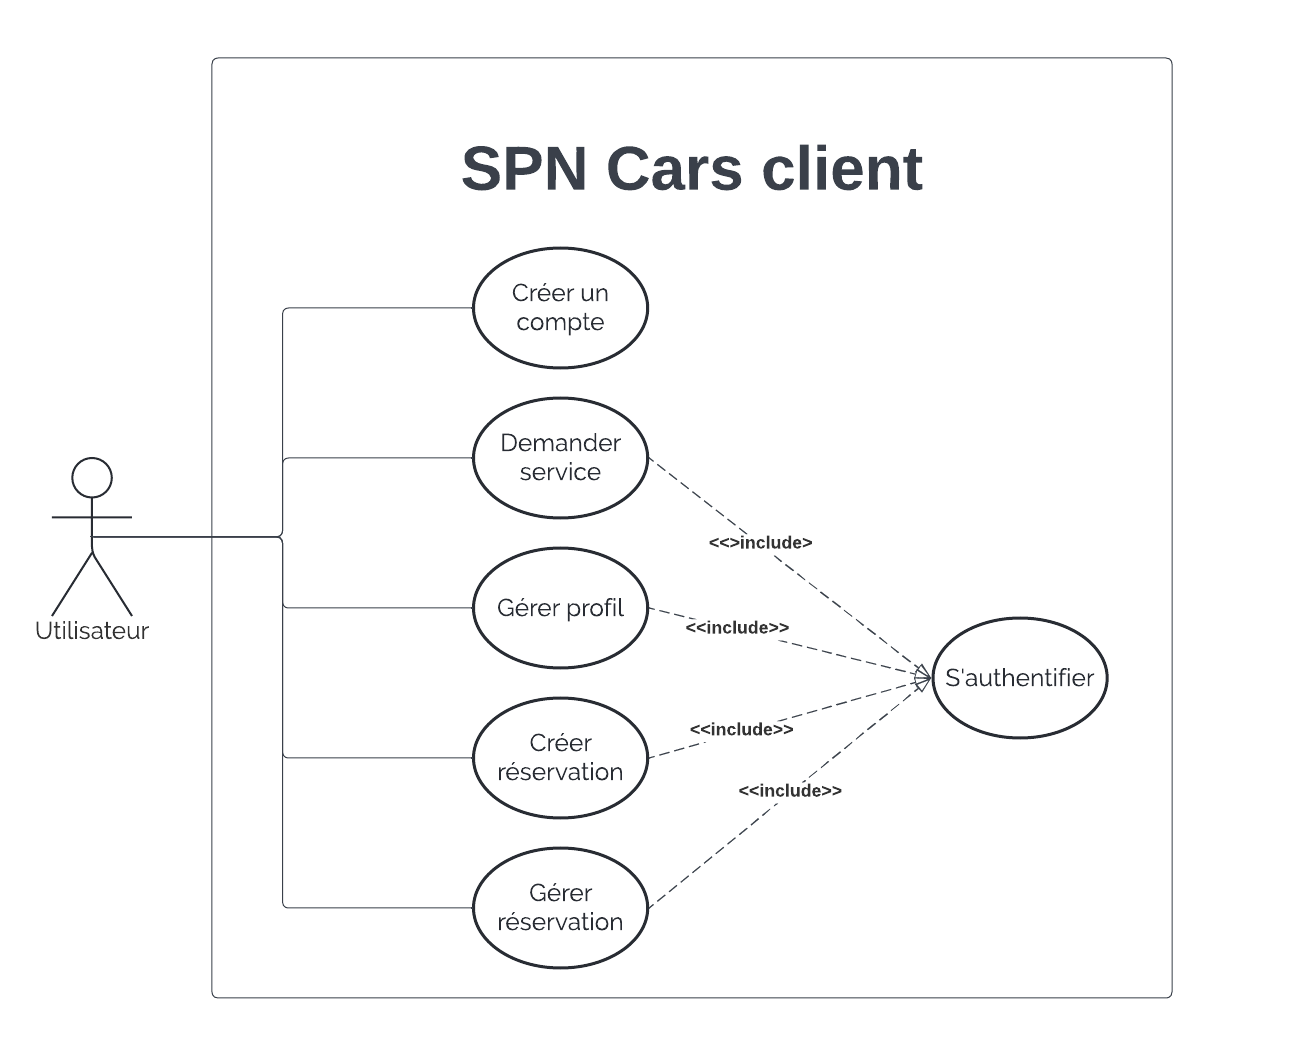
\includegraphics[height=0.8\textheight]{uml/use_cases.png}
    \vspace{1cm}
    \caption{Diagramme de cas d'utilisation}
    \label{fig:use_case_diag}
\end{figure}

\subsubsection{Diagramme de classes}
\begin{figure}[H]
    \centering
    \rotatebox[origin=c]{-90}{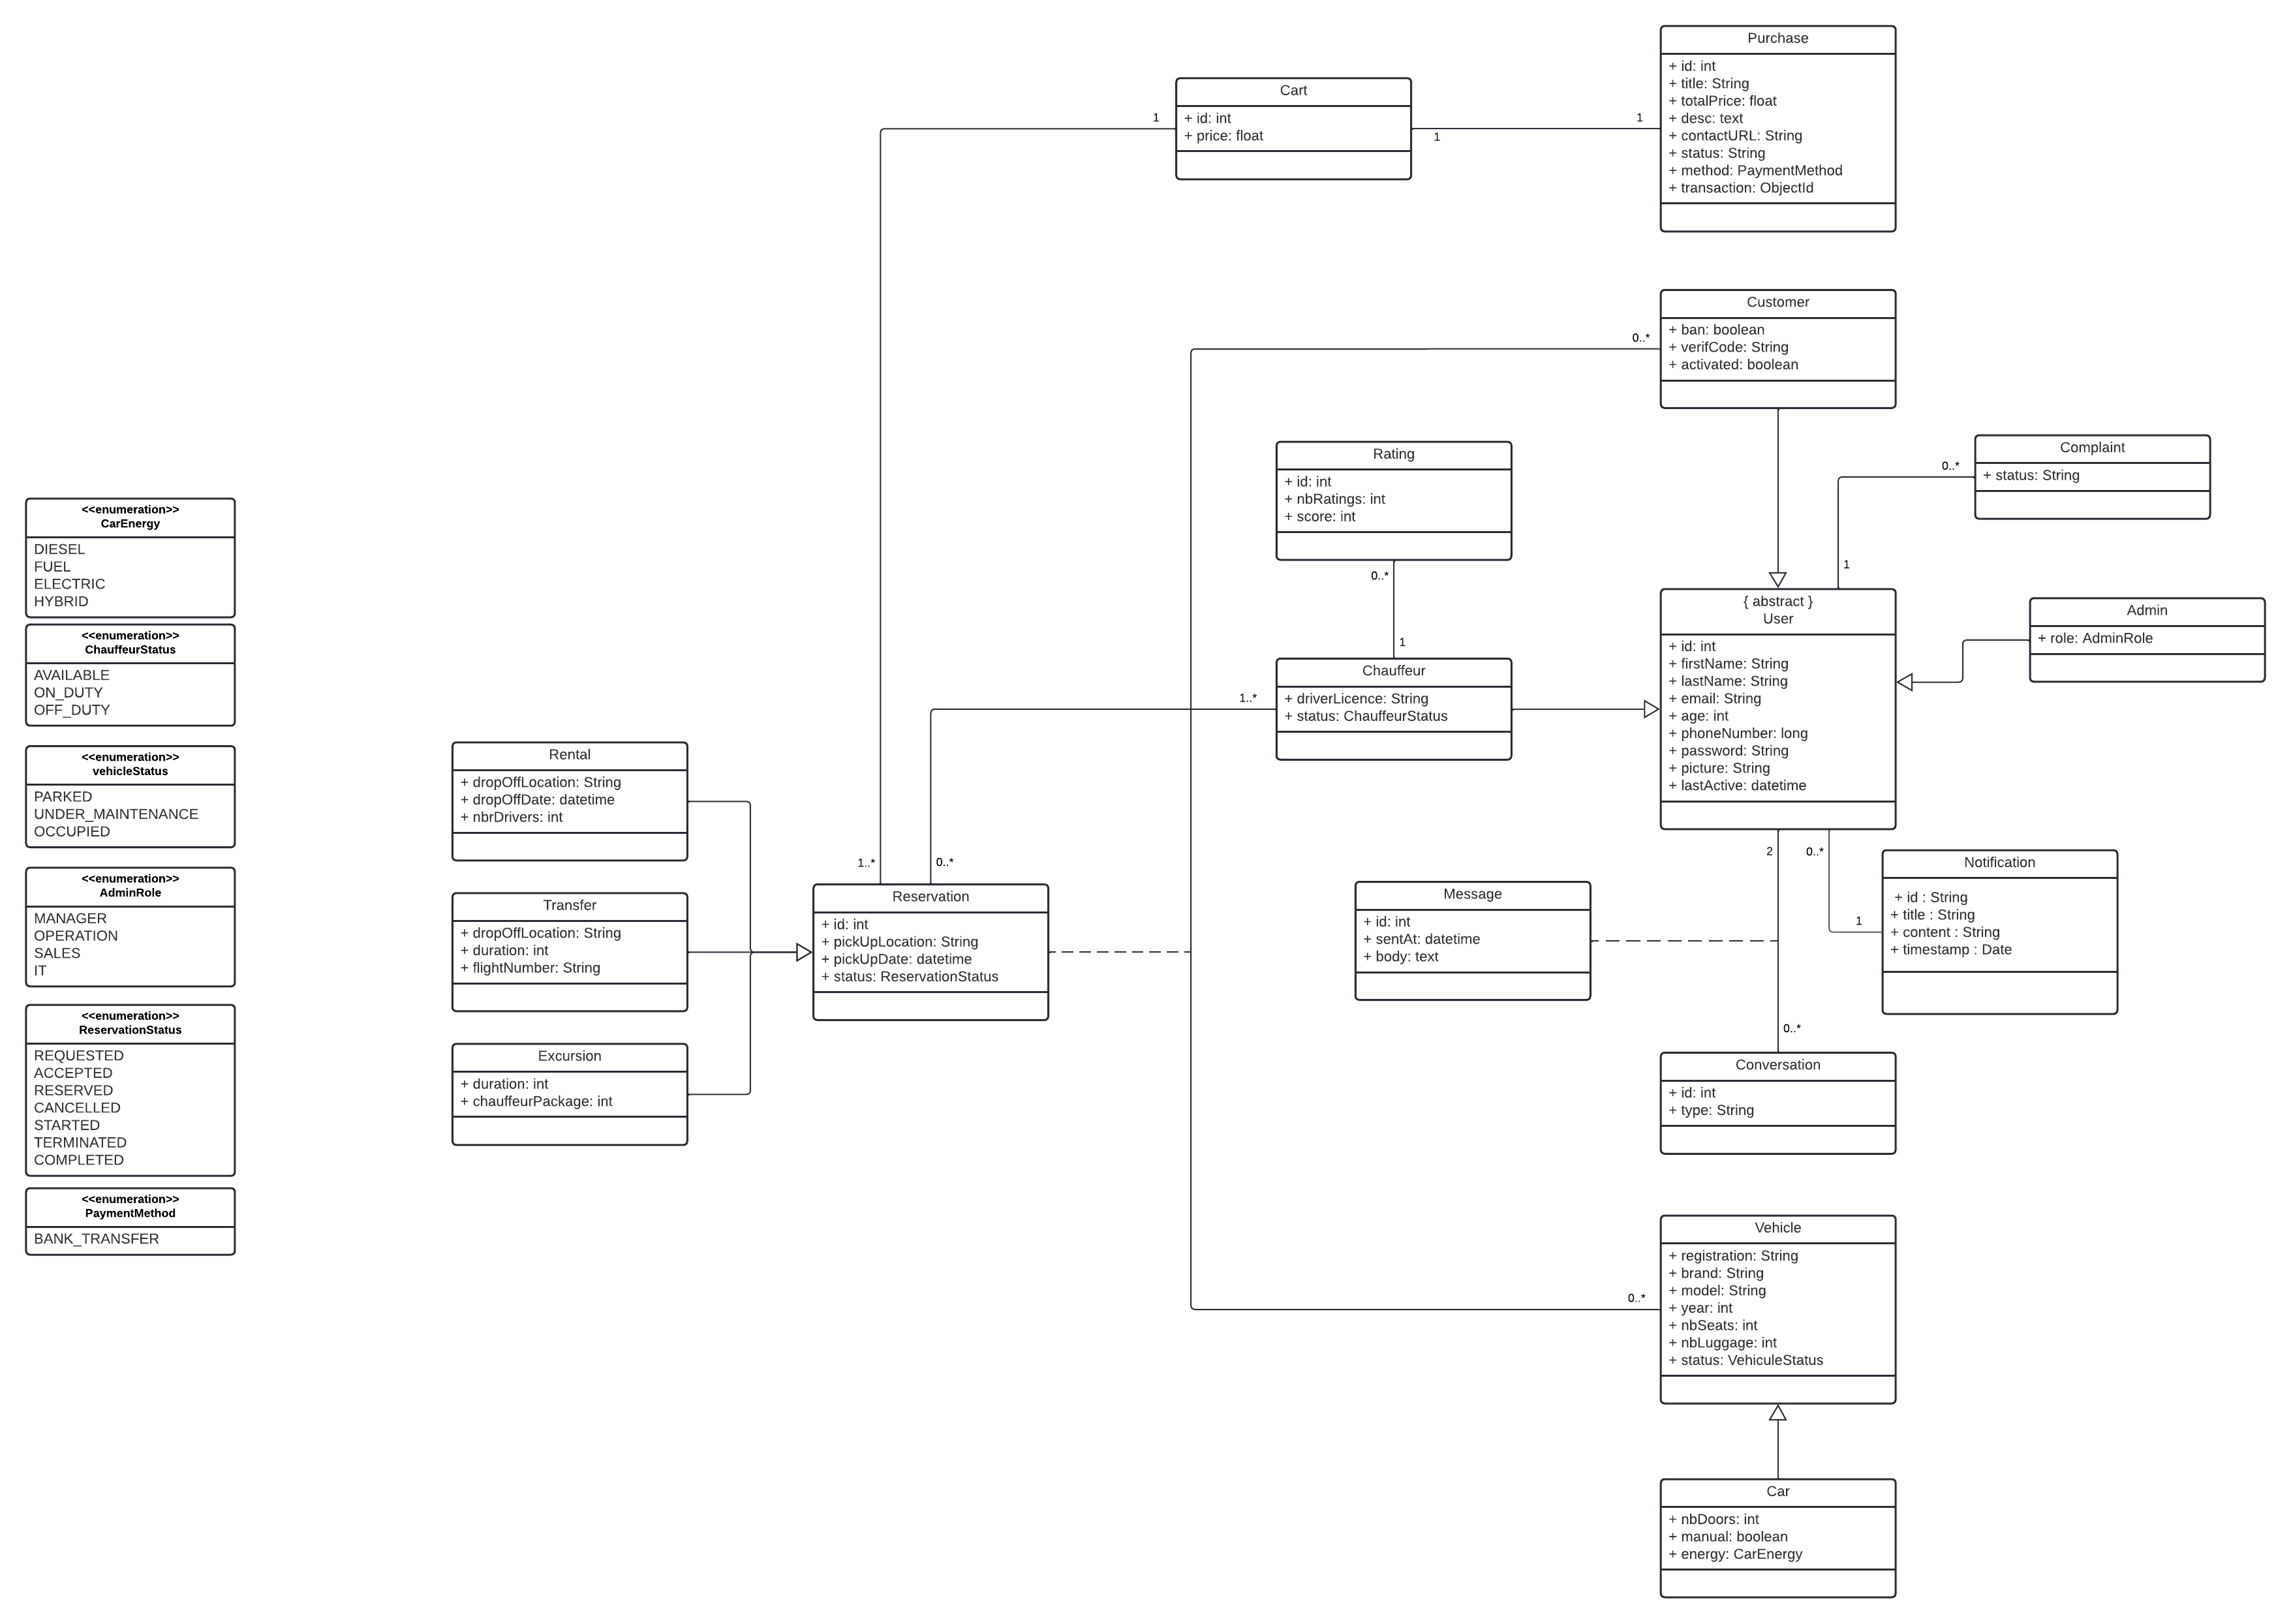
\includegraphics[width=1.2\textwidth]{uml/class_diag.png}}
    \vspace{1cm}
    \caption{Diagramme de classe}
    \label{fig:class_diag}
\end{figure}
\subsubsection{Diagramme de séquences}
Les diagrammes de séquences présenteront le fonctionnement de l'application dès l'authentification jusqu'au fonctionnalités les plus complexes.
\paragraph{L'authentification}\mbox{} \\
L'authentification est la première étape dans le cycle de vie de l'application, lors du premier démarrage de l'application il est nécessaire de vérifier si l'utilisateur à déja connecté sur l'application.\\
\noindent Cette étape est nécessaire pour réduire le nombre de connexion et faciliter l'expérience des utilisateurs.
\vspace{1cm}
\begin{figure}[H]
    \centering
    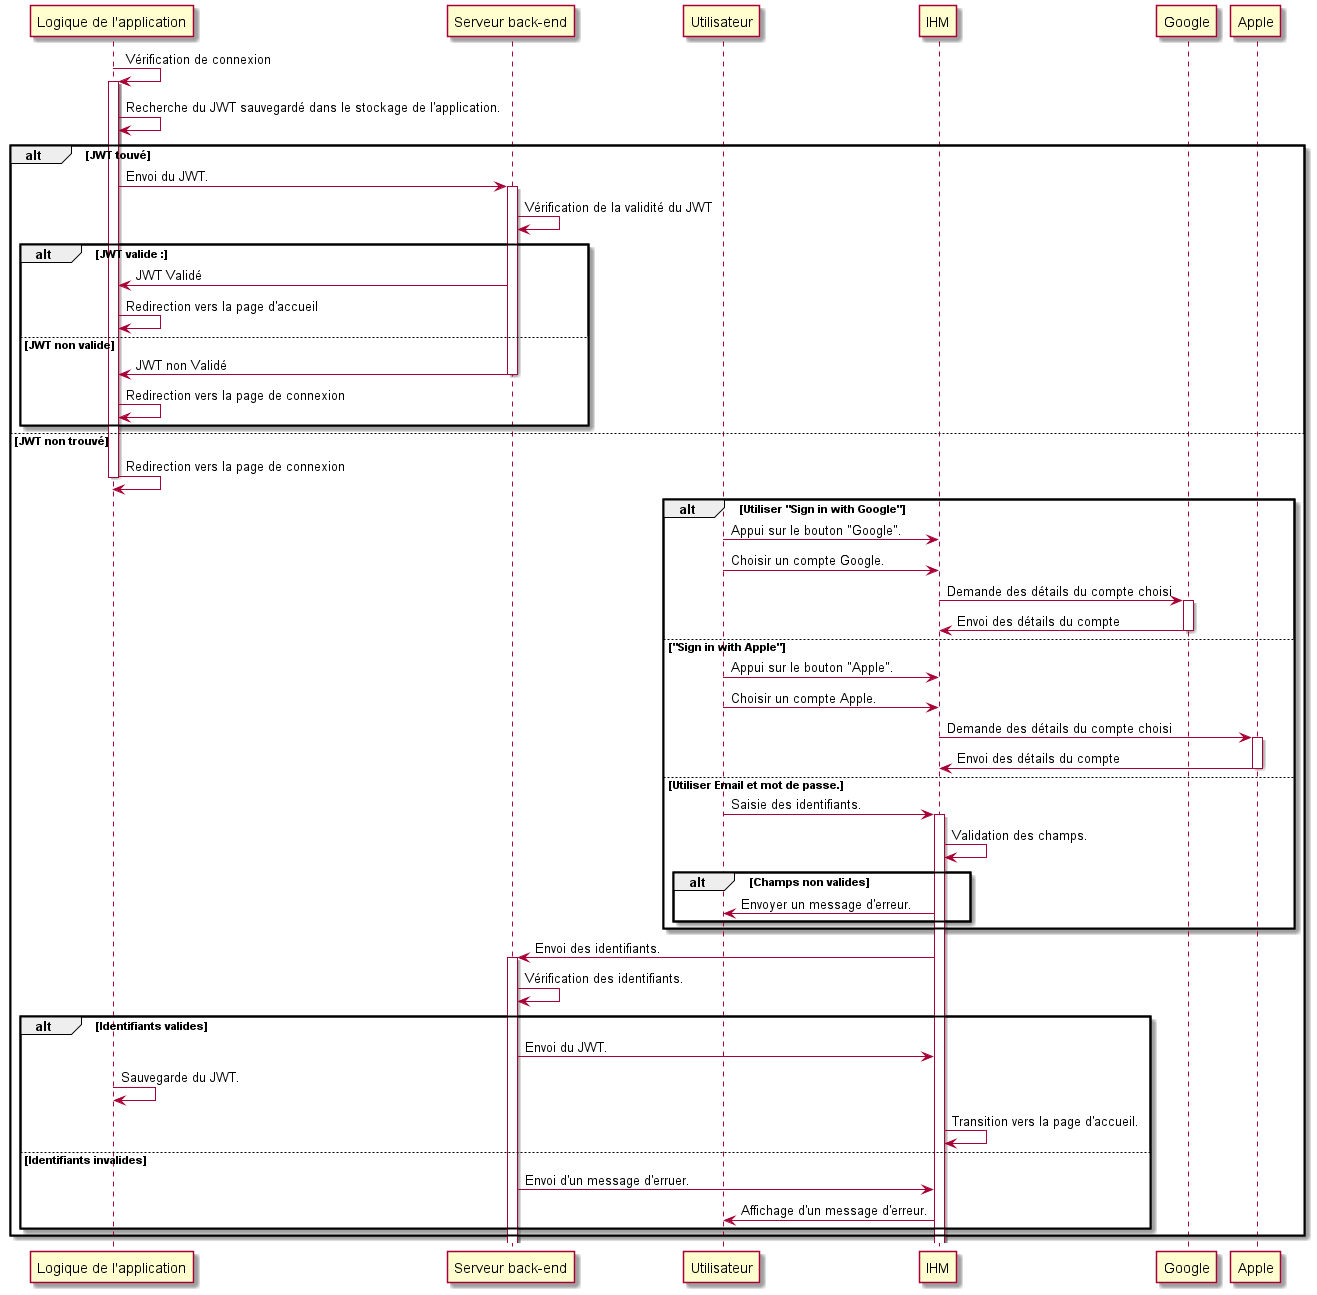
\includegraphics[width = \textwidth]{uml/Authentification.png}
    \vspace{1cm}
    \caption{Diagramme de séquences: Authentification}
    \label{fig:seq_auth}
\end{figure}
\paragraph{Demander un service}\mbox{} \\
Pour louer une voiture, l'utilisateur a besoin de spécifier tout d'abord les paramètres suivants :
\begin{itemize}
    \item Le type de service demandé (Location / Transfert / Excursion / Long Ride).
    \item L'adresse de départ.
    \item L'heure de départ.
    \item L'adresse d'arrivée (Pas toujours disponible selon le type de service).
    \item L'heure d'arrivée (Pas toujours disponible selon le type de service).
    \item La durée du service demandé (Pas toujours disponible selon le type de service).
\end{itemize}
\vspace{1cm}
\begin{figure}[H]
    \centering
    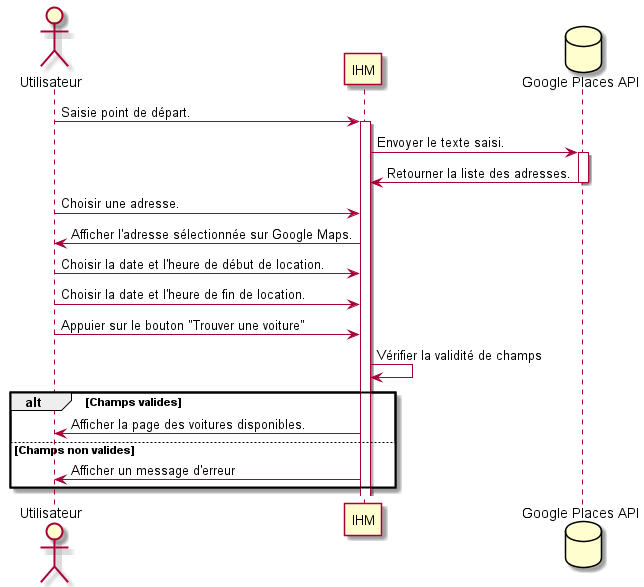
\includegraphics[width = \textwidth]{uml/rent a car.png}
    \vspace{1cm}
    \caption{Diagramme de séquences: Demander une location.}
    \label{fig:seq_location}
\end{figure}
\vspace{1cm}
\begin{figure}[H]
    \centering
    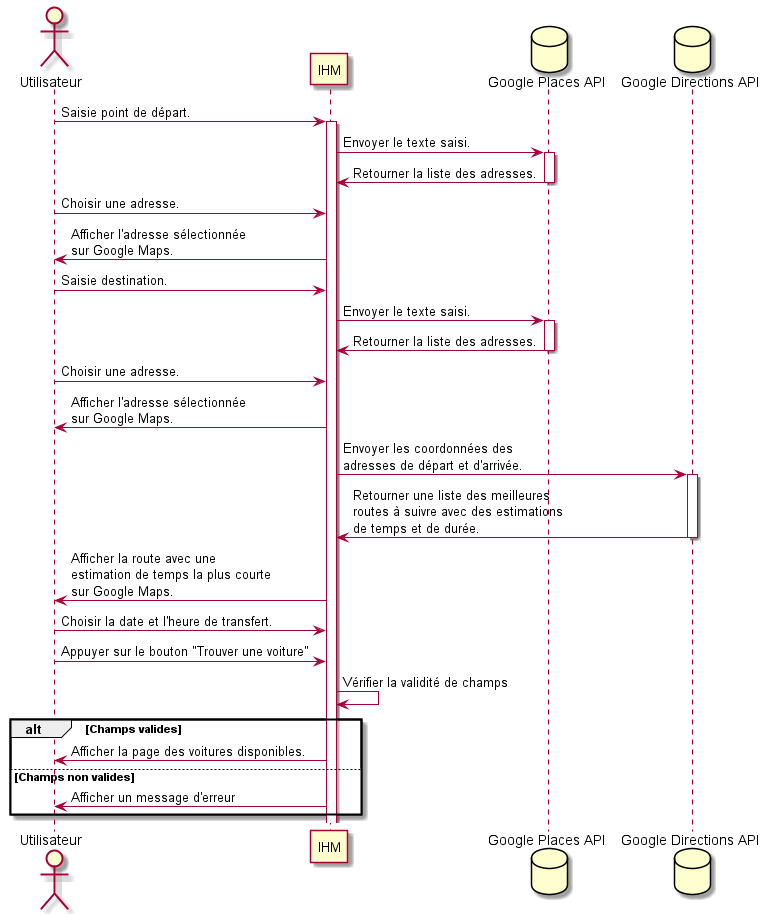
\includegraphics[width = \textwidth]{uml/transfert.png}
    \vspace{1cm}
    \caption{Diagramme de séquences: Demander un transfert.}
    \label{fig:seq_transfert}
\end{figure}
\paragraph{Affichage des voitures disponibles} \mbox{}\\
Après sélection des informations nécessaires par l'utilisateur, une recherche des voitures qui répondent aux critères de recherche choisis. Une fois une liste de voitures est prête, les voitures seront affichés. L'utilisateur peut appuyer sur une voiture pour découvrir ses caractéristiques et choisir ensuite de la louer ou continuer sa recherche.
Le diagramme suivant explique la procédure de la sélection de voitures.
\vspace{1cm}
\begin{figure}
    \centering
    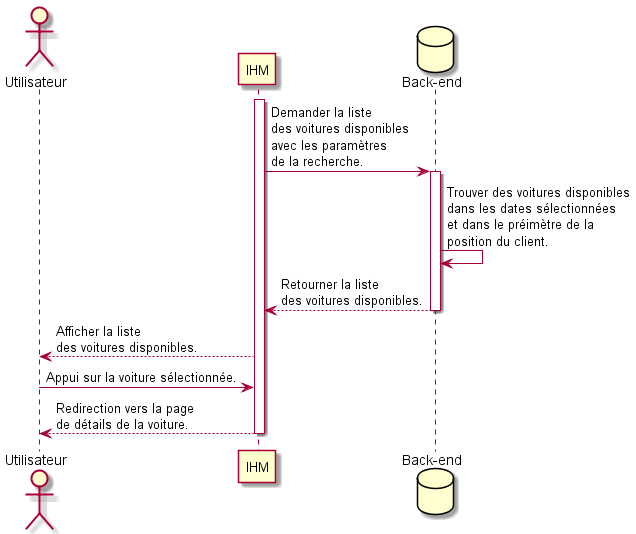
\includegraphics[width = \textwidth]{uml/choisir voiture.png}
    \vspace{1cm}
    \caption{Diagramme de séquences : Choisir une voiture}
    \label{fig:seq_car_select}
\end{figure}
\subsection{UI/UX Design}
Avant de passer au développement de l'application, il faut créer d'abord les prototypes des interfaces utilisateur. \\
\noindent Cette étape est nécessaire pour tester plusieurs approches dans les interfaces de l'application, s'assurer d'offrir une expérience utilisateur agréable. \\
\vspace{1cm}
\begin{multicols}{2}
    \begin{figure}[H]
        \centering
        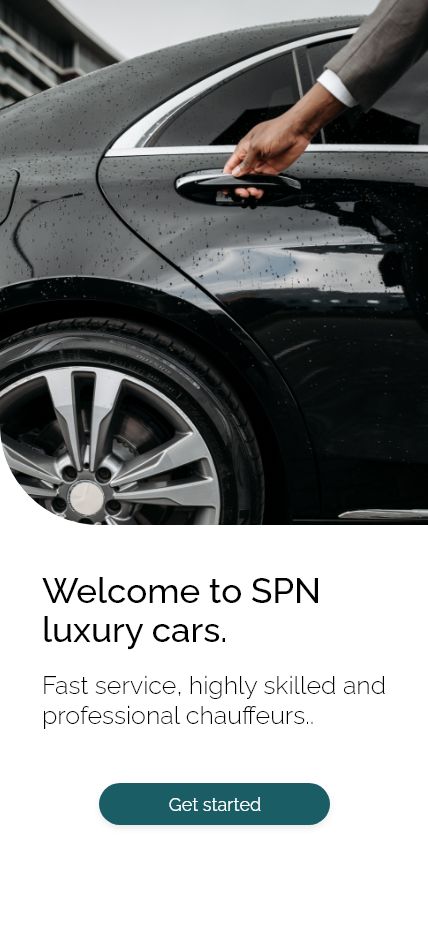
\includegraphics[width=0.25\textwidth]{ui_screenshots/Guide.png}
        \vspace{1cm}
        \caption{Première page.}
        \label{fig:start_page}
    \end{figure}
    \begin{figure}[H]
        \centering
        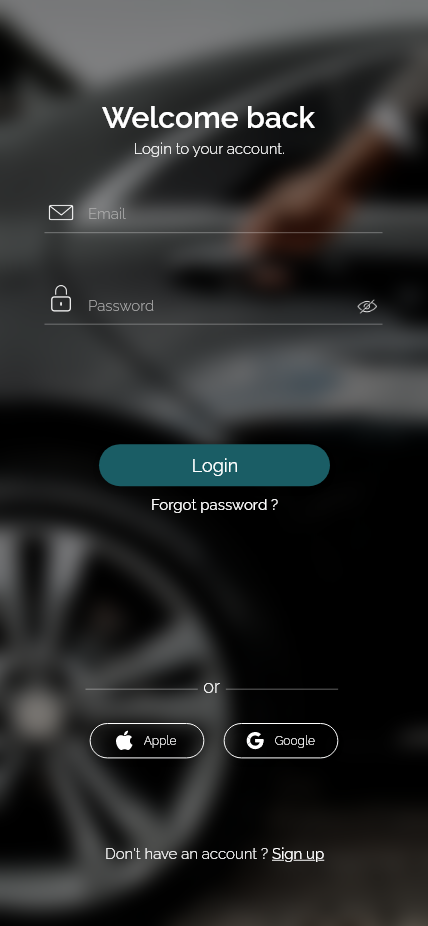
\includegraphics[width=0.25\textwidth]{ui_screenshots/sign in.png}
        \vspace{1cm}
        \caption{Page de connexion.}
        \label{fig:sign_in_page}
    \end{figure}
\end{multicols}
\newpage
\begin{multicols}{2}
    \begin{figure}[H]
        \centering
        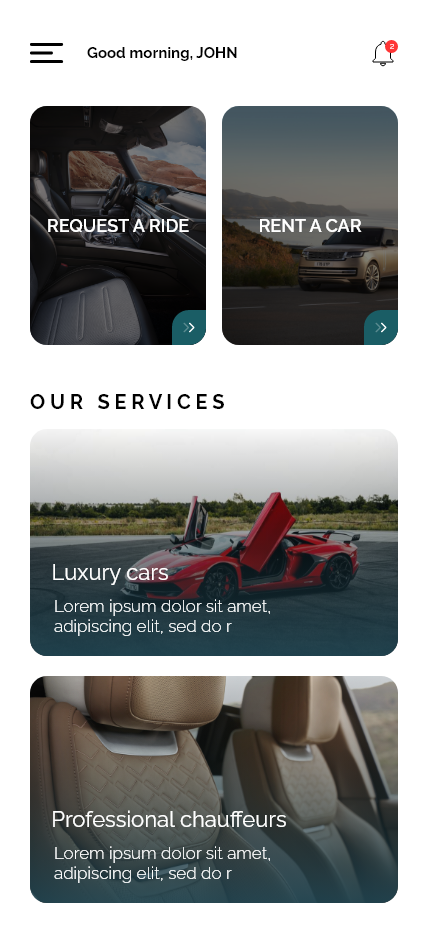
\includegraphics[width=0.25\textwidth]{ui_screenshots/No Active trip.png}
        \vspace{1cm}
        \caption{\centering Page d'accueil.}
        \label{fig:no_active_trip}
    \end{figure}
    \begin{figure}[H]
        \centering
        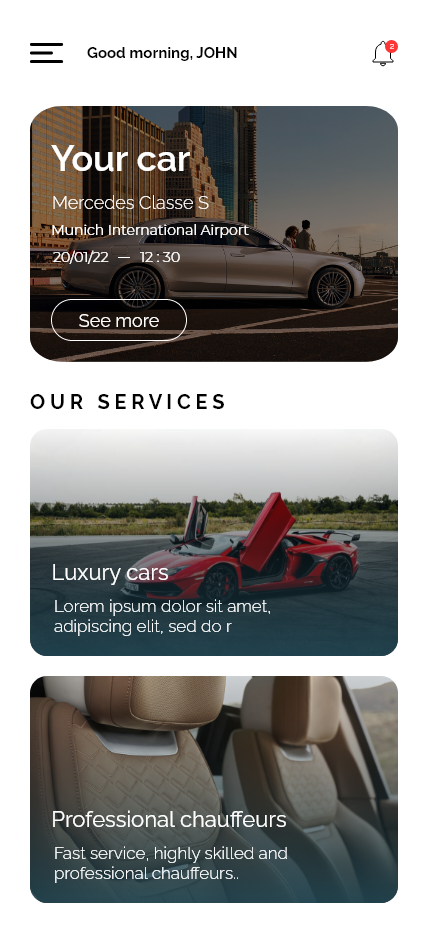
\includegraphics[width=0.25\textwidth]{ui_screenshots/Active trip.png}
        \vspace{1cm}
        \caption{\centering Page d'accueil lors d'un transfert en cours.}
        \label{fig:active_trip}
    \end{figure}
\end{multicols}
\begin{multicols}{2}
    \begin{figure}[H]
        \centering
        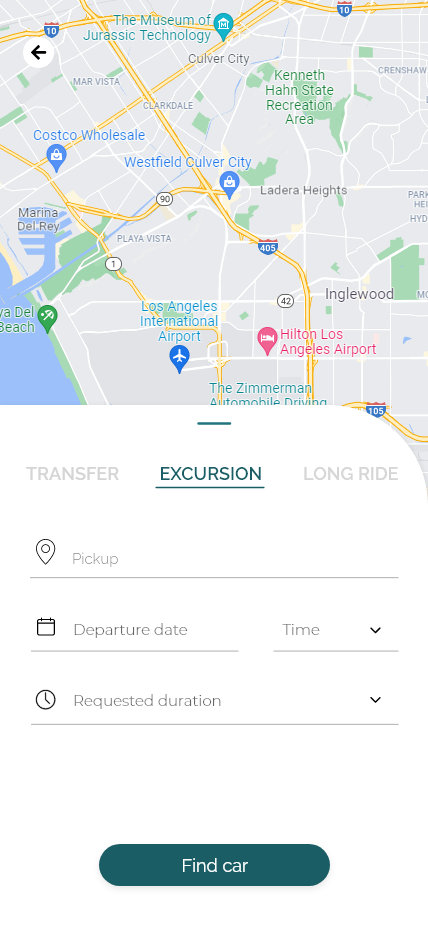
\includegraphics[width=0.25\textwidth]{ui_screenshots/Excursion.png}
        \vspace{1cm}
        \caption{\centering Sélection de type de transfert.}
        \label{fig:trip_select}
    \end{figure}
    \begin{figure}[H]
        \centering
        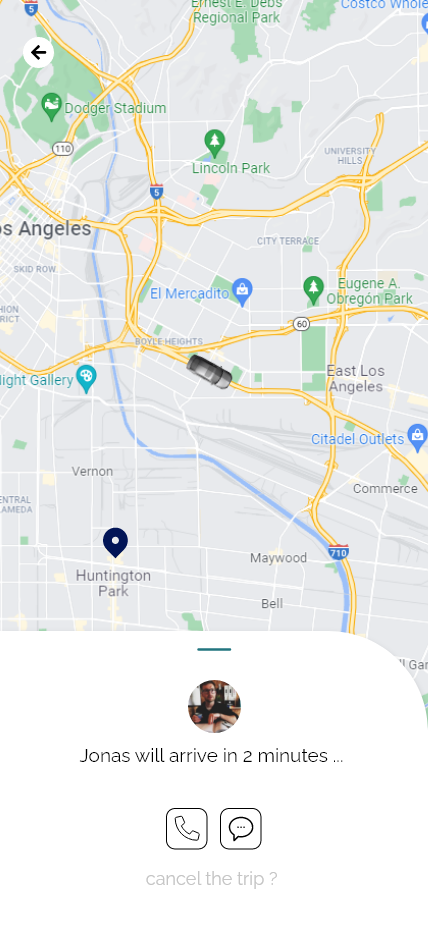
\includegraphics[width=0.25\textwidth]{ui_screenshots/Map view.png}
        \vspace{1cm}
        \caption{\centering Suivi de la position actuelle du chauffeur avec la voiture.}
        \label{fig:follow_driver}
    \end{figure}
\end{multicols}
\newpage
\begin{multicols}{2}
    \begin{figure}[H]
        \centering
        \includegraphics[width=0.25\textwidth]{ui_screenshots/Available cars – 1.png}
        \vspace{1cm}
        \caption{\centering Liste de voitures disponibles.}
        \label{fig:available_cars}
    \end{figure}
    \begin{figure}[H]
        \centering
        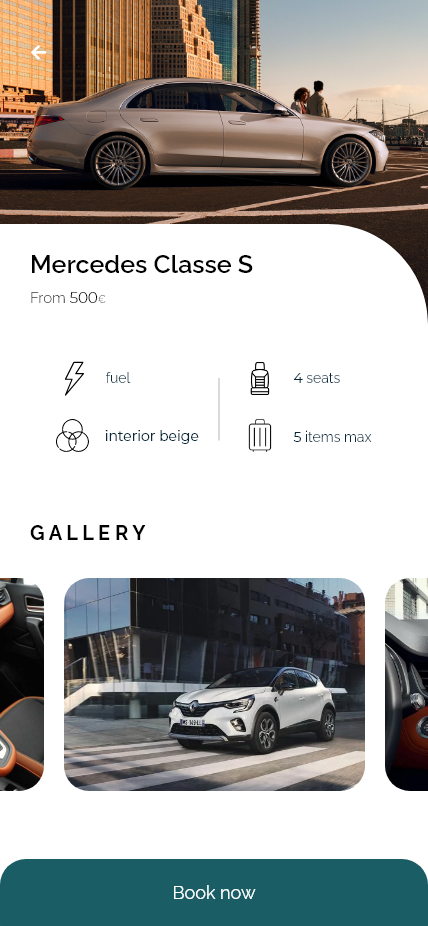
\includegraphics[width=0.25\textwidth]{ui_screenshots/Car details.png}
        \vspace{1cm}
        \caption{\centering Détails de la voiture sélectionnée.}
        \label{fig:car_details}
    \end{figure}
\end{multicols}
\vspace{1cm}
\begin{figure}[H]
    \centering
    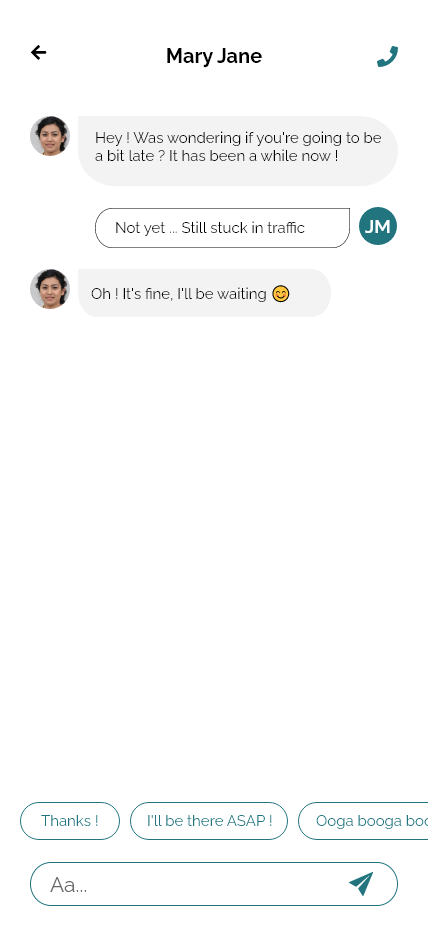
\includegraphics[width=0.25\textwidth]{ui_screenshots/DMs.png}
    \vspace{1cm}
    \caption{\centering Messagerie instantannée avec le chauffeur.}
    \label{fig:dms}
\end{figure}

\subsection{Technologies et logiciels utilisés}
Comme cette application sera une application mobile, il est nécessaire que la performance soit la priorité lors du développement. C'est porquoi on a choisi les technologies suivantes pour offrir une application rapide, performante, facile à utiliser.\\
\noindent Ses différentes technologies sont classifiés dans trois domaines principalement : Conception des interfaces graphiques, développement de l'application, et développement du back-end de l'application.\\
\paragraph{Adobe Xd}\mbox{} \\
\vspace{1cm}
\begin{figure}[H]
    \centering
    
\includegraphics[width=0.25\textwidth]{xd_logo.png}
    \vspace{1cm}
    \caption{Logo Adobe Xd}
    \label{fig:xd_logo}
\end{figure}
\textit{\textbf{Adobe Xd}} est un outil de conception et modélisation des interfaces utilisateur des applications web et mobiles, développé par Adobe Inc.\\
\noindent Grâce aux outils fournis par Adobe Xd, la conception, l'amélioration et la rectification des interfaces graphiques et l'expérience de l'utilisateur de l'application sera plus facile, plus rapide et plus efficace.
\noindent Dans le cadre de ce projet, Adobe Xd a été utilisé pour la création des prototypes des interfaces graphiques, qui seront, par la suite, construits en application mobile à l'aide de Flutter.
\paragraph{Flutter}\mbox{} \\
\vspace{1cm}
\begin{figure}[H]
    \centering
    
\includegraphics[width=0.25\textwidth]{flutter.png}
    \vspace{1cm}
    \caption{Logo Flutter}
    \label{fig:flutter_logo}
\end{figure}
\textit{\textbf{Flutter}} est un kit de développement (SDK) open-source créé par Google et publié en 2017.\\
\noindent Flutter permet de créer des application mobiles (Android / iOS), web et meême desktop (Windows / Linux / MacOS), avec une seule base de code en Dart, un langage de programmation développé aussi par Google. \\
\noindent Flutter présente plusieurs avantages qui permettent de créer des applications mobiles performantes et réduit aussi le coût et le temps de développement nécessaires, grâce au langage de programmation utilisé \textit{\textbf{Dart}} qui est très facile à maitriser et qui offre plusieurs avantages, dont le plus important la fonctionnalité de <<\textit{\textbf{Hot Reload}}>> qui permet de recharger l'application et afficher les changements sur l'écran sans passer par la recompilation du code source.
\paragraph{Express JS}\mbox{} \\
\vspace{1cm}
\begin{figure}[H]
    \centering
    
\includegraphics[width=0.25\textwidth]{express.png}
    \vspace{1cm}
    \caption{Logo Express}
    \label{fig:express_logo}
\end{figure}
\textit{\textbf{Express JS}} est un framework back-end gratuit et open-source pour NodeJS.\\
\noindent Créé par TJ Holowaychuk, la première version publique d'Express JS a été introduite au public en 2010.
\paragraph{MongoDB} \mbox{} \\
\vspace{1cm}
\begin{figure}[H]
    \centering
    
\includegraphics[width=0.25\textwidth]{mongo.png}
    \vspace{1cm}
    \caption{Logo MongoDB}
    \label{fig:mongo_logo}
\end{figure}
\paragraph{Firebase} \mbox{} \\
\vspace{1cm}
\begin{figure}[H]
    \centering
    
\includegraphics[width=0.25\textwidth]{firebase.png}
    \vspace{1cm}
    \caption{Logo Firebase}
    \label{fig:firebase_logo}
\end{figure}
\paragraph{Git} \mbox{} \\
\vspace{1cm}
\begin{figure}[H]
    \centering
    
\includegraphics[width=0.25\textwidth]{git.png}
    \vspace{1cm}
    \caption{Logo Git}
    \label{fig:git_logo}
\end{figure}

